\documentclass[pdflatex,sn-mathphys-num]{sn-jnl}

\usepackage{amssymb}

\usepackage{placeins}
\usepackage{microtype}
% Note: amsmath, amssymb, graphicx, booktabs, and hyperref are natively loaded or handled by sn-jnl.

\newcommand{\PEHE}{\mathrm{PEHE}}
\newcommand{\E}{\mathbb{E}}

\begin{document}

\title[Geometry-Dependent Rankings of CATE Estimators]{Geometry-Dependent Rankings of CATE Estimators and the Information Cost of Performance Recovery under Pure Effect-Surface Shift}

\author*[1]{\fnm{Negar} \sur{Rezaei}}\email{n\_rezaei@mathdep.iust.ac.ir}
\author[1]{\fnm{Ehsan} \sur{Moeini}}\email{ehsan\_moeini@mathdep.iust.ac.ir}

\affil*[1]{\orgdiv{School of Mathematics \& Computer Science}, \orgname{Iran University of Science and Technology}, \city{Tehran}, \country{Iran}}

\abstract{The relative performance of conditional average treatment effect (CATE) estimators depends systematically on the effect surface geometry $\tau(x)$. Standard benchmarks often confound this geometry with dimension, overlap, and noise. Isolating pure geometry variation in synthetic designs, we document stable ranking reversals: tree-based methods dominate threshold surfaces at all signal levels, whereas neural architectures excel on interaction surfaces at moderate-to-high signal levels, and on smooth surfaces only at the highest signal level. Using a two-expert mixture as an analytical probe on a shifted interaction geometry, we observe a PEHE of $1.26$—worse than both a constant-ATE ($1.01$) and a null predictor ($1.10$). Given the intrinsic failure of the base experts, observable routing mechanisms cannot recover performance. Mapping target label budgets ($m$) reveals that factual-only fine-tuning is ineffective at small $m$, while direct $\tau$-labels become beneficial only for $m \gtrsim 50$. Even under favorable supervision, a target-only T-learner remains highly competitive. Supported by synthetic evidence, these findings reframe adaptive CATE estimation as an information-bounded problem rather than a matter of label-free robustness.}


\keywords{CATE estimation, effect-surface geometry, few-shot adaptation, heterogeneous treatment effects, inductive bias, pure geometry shift}

\maketitle

\section{Introduction}
\label{sec:intro}

Estimating conditional average treatment effects (CATE) is central to personalized decision-making in medicine, economics, and public policy. A wide range of estimators is available, including meta-learners \citep{kunzel2019,nie2021,kennedy2023}, causal forests \citep{wager2018,athey2019}, Bayesian additive regression trees \citep{hill2011,chipman2010}, and neural representation networks \citep{shalit2017,johansson2016,shi2019}. These methods encode distinct structural assumptions about the effect surface \citep{curth2021}. Tree-based methods are expected to perform well on piecewise-constant, axis-aligned surfaces, whereas neural networks are expected to suit smooth or interacting surfaces. If these inductive biases hold, no single estimator family should dominate across all geometries of $\tau(x)=\mathbb{E}[Y(1)-Y(0)\mid X=x]$.

Existing benchmarks rarely isolate the functional form of the effect surface. Public datasets \citep{hill2011,dorie2019} and large-scale model-selection studies \citep{mahajan2024} typically report performance within fixed data-generating processes or averaged across heterogeneous settings. In such regimes, the geometry of $\tau(x)$ remains entangled with covariate dimension, overlap, and noise level, so observed rankings may be artifacts of the particular process chosen \citep{curth2021benchmark}.

The issue is also of practical importance. An estimator is frequently trained or selected on one population and subsequently deployed on another. When an unrecorded effect modifier (for example, a measure of disease severity) is distributed differently across the two populations, the conditional effect surface given the observed covariates changes, even if the covariate law $P(X)$ and the propensity score $e(x)$ remain identical. We refer to such a change as a \emph{pure geometry shift}. Because the true effects are never observed in real data, the performance cost of this shift cannot be measured directly.

We therefore construct controlled designs in which only the functional form of $\tau(x)$ varies. Covariates, propensity scores, baseline outcomes, and noise are held fixed; the effect surface is smooth, axis-aligned threshold, or interaction. A semi-synthetic variant that retains real covariates is also examined. With ground-truth $\tau$ available throughout, we address three precise questions:
\begin{enumerate}
  \item[\textbf{Q1}] Do estimator rankings and the reliability of selection criteria that need no counterfactuals, depend on the geometry of $\tau$?
  \item[\textbf{Q2}] How much accuracy does a model lose when the geometry changes between source and target, and does a router that sees only observable signals help?
  \item[\textbf{Q3}] How much target supervision is needed to recover, and does the answer depend on the type of supervision?
\end{enumerate}

\paragraph{Contributions}
\begin{itemize}
  \item \emph{Geometry-dependent ranking reversals.} On threshold surfaces, the X-learner and causal forests achieve the lowest PEHE in all 10 seeds at every signal level examined. Neural architectures lead on interaction surfaces at moderate-to-high signal levels, and on smooth surfaces only at the highest signal level. Along a continuous smooth-to-threshold path the relative ordering of a neural and a tree-biased expert reverses, with the tree expert ahead in all ten seeds by the midpoint (Section~\ref{sec:reversal}). Counterfactual-free selection criteria identify the best of four estimators less frequently on interaction surfaces, although their regret remains small (App.~B).
  \item \emph{Failure of observable routing under pure geometry shift.} Using a two-expert mixture as an analytical probe trained on source geometries $\{A,B\}$ and evaluated on a shifted interaction geometry $C$, we observe a PEHE of $1.26$—worse than both a constant-ATE predictor ($1.01$) and a null predictor ($1.10$). Given the intrinsic failure of the base experts, observable routing mechanisms cannot recover performance. In a separate study, a router trained on one regime performs worse on another than the best single estimator selected in hindsight on every tested pair (Sections~\ref{sec:gap} and~\ref{sec:neg}).
  \item \emph{Information cost of recovery.} Direct $\tau$-labels, although typically unavailable in practice, become clearly beneficial only for $m\gtrsim 50$. Doubly robust pseudo-labels, constructed from the entire target pool and therefore not budget-matched, remain near the constant baseline. A pure target-only T-learner trained on the 1400 target factual units, with no source model, reaches PEHE $0.47$ (Section~\ref{sec:ladder}).
  \item \emph{Exploratory negative results.} A train-only geometry score tracks the performance margin between tree-based and neural estimators along the synthetic continuum (Pearson $r=-0.71$, 25 runs) but predicts the winner on ACIC 2016 \citep{dorie2019} no better than the majority class (accuracy $0.61$ versus $0.78$ over 18 runs on six settings). Disagreement-based active selection does not improve upon random selection (Section~\ref{sec:neg}).
\end{itemize}
Section~\ref{sec:setup} details the experimental designs. Section~\ref{sec:instrument} describes the measurement instrument. Results appear in Sections~\ref{sec:reversal}--\ref{sec:neg}.

\section{Related work}

\subsection*{CATE estimators and their inductive biases}
Meta-learners \citep{kunzel2019,nie2021,kennedy2023}, causal forests \citep{wager2018,athey2019}, Bayesian additive regression trees (BART) \citep{hill2011,chipman2010}, and neural representation networks \citep{shalit2017,johansson2016,shi2019} impose different structures on the effect surface. \citet{curth2021} study how architectural inductive biases, such as sharing structure between the outcome surfaces, affect neural CATE learners. Outside causal inference, tree ensembles often outperform neural networks on tabular data with irregular target functions \citep{grinsztajn2022}. We do not propose a new architecture; we vary only the shape of $\tau(x)$ and measure how estimator rankings change.

\subsection*{Benchmarking and model selection}
CATE benchmarks usually compare estimators within fixed data-generating processes \citep{dorie2019,curth2021benchmark}, and \citet{curth2021benchmark} argue that conclusions are sensitive to the process chosen. Without counterfactuals, candidate models are compared with surrogate risks such as factual outcome error, inverse-propensity-weighted (IPW) residuals, doubly robust scores, and influence-function-based validation \citep{rolling2014,schuler2018,saito2020,alaa2019}; \citet{mahajan2024} benchmark many of these at scale. We ask a narrower question: how the reliability of such surrogates varies with the geometry of $\tau(x)$ when everything else is held fixed (App.~B).

\subsection*{Distribution shift and transfer for treatment effects}
Work on transporting or generalizing causal effects typically concerns changes in the covariate distribution or in the treatment-assignment mechanism between populations \citep{pearl2011,bareinboim2016,dahabreh2019}; for instance, \citet{kyono2023} select effect models for domain adaptation using causal knowledge. Transfer learning has also been used to estimate effects from a few target units \citep{kunzel2018}. We consider a different case in which $P(X)$, $e(x)$, and the control-arm outcome function are unchanged and only the treated-arm response, hence $\tau(x)$, shifts. Consequently, we measure how recovery depends on the supervision available in the target.

\subsection*{Positioning}
To our knowledge, studies on model selection and transfer learning have not varied the shape of $\tau(x)$ in isolation, nor have they compared few-shot adaptation against constant and target-only learners. Our contribution is a controlled characterization of these two points, not a new estimator.

\section{Problem setting and experimental designs}
\label{sec:setup}

\subsection{Estimand, metric, and notation}
Let $X\in\mathbb R^p$ be covariates, $T\in\{0,1\}$ a binary treatment, and $Y=TY(1)+(1-T)Y(0)$ the observed outcome. Under the stable unit treatment value assumption (SUTVA), unconfoundedness ($\{Y(0),Y(1)\}\perp T\mid X$), and positivity ($0<e(x)<1$ with $e(x)=P(T=1\mid X=x)$), the CATE is identified:
\begin{equation}
\tau(x)=\E[Y(1)-Y(0)\mid X=x]=\E[Y\mid X=x,T=1]-\E[Y\mid X=x,T=0].
\end{equation}
Write $\mu_t(x)=\E[Y(t)\mid X=x]$, so that $\tau=\mu_1-\mu_0$. We measure accuracy by the root precision in estimation of heterogeneous effects \citep{hill2011},
\begin{equation}
\PEHE(\hat\tau)=\sqrt{\E_X\big[(\hat\tau(X)-\tau(X))^2\big]},
\end{equation}
estimated on held-out units and referred to simply as PEHE; some papers report its square. Two reference predictors set the scale. The constant $\hat\tau\equiv\E[\tau(X)]$, the best constant, has PEHE $\mathrm{sd}(\tau(X))$ but requires the true average effect, so it is an oracle. The zero-effect predictor $\hat\tau\equiv 0$ requires nothing and has PEHE $\sqrt{\mathrm{sd}(\tau(X))^2+(\E[\tau(X)])^2}$.

\subsection{Effect-surface geometry and geometry shift}
By \emph{geometry} we mean the functional form of $\tau:\mathbb R^p\to\mathbb R$: whether it is smooth, piecewise constant along coordinate axes, or driven by an interaction. A \emph{geometry shift} is a change between a source and a target population,

\begin{equation}
\label{eq:geometry-shift}
\begin{aligned}
P_{\mathrm{src}}(X)
    &= P_{\mathrm{tgt}}(X),\\
e_{\mathrm{src}}(x)
    &= e_{\mathrm{tgt}}(x),\\
\mu_{0,\mathrm{src}}(x)
    &= \mu_{0,\mathrm{tgt}}(x),\\
\tau_{\mathrm{src}}(x)
    &\ne \tau_{\mathrm{tgt}}(x).
\end{aligned}
\end{equation}

so that only the treated-arm response $\mu_1=\mu_0+\tau$ changes. No signal from covariates, propensities, or control outcomes reveals such a shift, and it can be detected only from target outcomes of treated units. The motivating mechanism is an unrecorded effect modifier whose distribution differs across the two populations.

\subsection{Synthetic geometries}
Covariates are $X\sim\mathcal N(0,I_{12})$, and treatment is $T\sim\mathrm{Bernoulli}(e(X))$ with $e(x)=\sigma(0.4x_1-0.3x_2+0.2x_3)$, where $\sigma$ is the logistic function (propensities lie between about $0.08$ and $0.91$). The outcome is generated as ${Y=\mu_0(X)+T\,\tau(X)+\varepsilon}$, with $\varepsilon\sim\mathcal N(0,0.5^2)$ and $\mu_0(x)=0.5x_1+0.3x_2-0.2x_4+0.1x_1x_2$. Only $\tau$ differs across regimes:
\begin{align}
\tilde\tau_A(x)&=\tanh(0.8x_1+0.5x_2)+0.4\sin x_3+0.3x_5,\\
\tilde\tau_B(x)&=\mathbf 1\{x_1>0,\;x_2>-0.5\}+0.5\cdot\mathbf 1\{x_3>0.5\}-0.3\cdot\mathbf 1\{x_1\le 0\},\\
\tilde\tau_C(x)&=\tanh(x_1)\,x_2+0.4x_3^2-0.2x_4,
\end{align}
and $\tau_g(x)=s\,\tilde\tau_g(x)/\hat\sigma_g$ with signal strength $s\in\{0.5,1,2\}$, where $\hat\sigma_g$ is the standard deviation of $\tilde\tau_g$ estimated once on $20{,}000$ draws, so that $\mathrm{sd}(\tau)\approx s$. Regime~A is smooth, Regime~B is piecewise constant with axis-aligned thresholds, and Regime~C combines a multiplicative interaction with quadratic and linear terms. Each surface depends on three or four of the twelve covariates, and the remaining covariates are noise. The effect modifiers $x_1$ to $x_3$ also drive treatment assignment. The standardized surfaces are correlated to different degrees (Monte Carlo estimates): $\mathrm{corr}(\tau_A,\tau_B)=0.70$, $\mathrm{corr}(\tau_B,\tau_C)=0.24$, and $\mathrm{corr}(\tau_A,\tau_C)=0.00$. The continuum is $\tau_\lambda=(1-\lambda)\tau_A+\lambda\tau_B$; it is not rescaled, so $\mathrm{sd}(\tau_\lambda)$ falls from $1.0$ at the endpoints to about $0.92$ at $\lambda=0.5$. Table~\ref{tab:design} lists sample sizes, splits, and seeds.

\subsection{Shift protocol and the IHDP-X benchmark}
The synthetic shift trains on $\{A,B\}$ and evaluates on $C$. Each source regime contributes the $70\%$ training split of an independent sample of $2000$ units (resulting in $1400$ units per regime, or $2800$ in total), and $12\%$ of the pooled units are held out for validation. The target is a fresh sample of $2000$ units of regime $C$, of which $1400$ form the adaptation pool and $600$ form the test set. At target time, the tree expert receives tree signals from tree models fitted on source data only, so a frozen model never uses a target outcome. Because $\mathrm{corr}(\tau_A,\tau_C)=0$, this is a strong shift: the source surfaces carry almost no linear information about the target surface.

\emph{IHDP-X} is a semi-synthetic benchmark built on the real covariates and treatment assignments of the IHDP replications of \citet{hill2011} in the form distributed with \citet{shalit2017} ($747$ units and $25$ covariates per replication). Baseline outcomes $\mu_0$ come from a ridge regression fitted to the observed control outcomes, and a base effect is the difference of two ridge fits to the treated and control units. The smooth surface is a distance-weighted $k$-nearest-neighbor ($k=40$) and ridge smoothing of this base effect. The threshold surface is a depth-3 decision tree on the three covariates most correlated with the base effect, whose leaves are set to levels $\pm3.0$ (plus a small within-leaf term), so it is close to a two-level step function. Both surfaces are standardized and scaled so that $\mathrm{sd}(\tau)=2.5$, and outcomes are re-simulated as $Y=\mu_0+T\,\tau+\varepsilon$ with $\varepsilon\sim\mathcal N(0,0.4^2)$. The two geometries were constructed to contrast strongly; thus, IHDP-X serves as a stress test rather than a naturally occurring shift. \newpage Source and target share the same units and differ only in $\tau$ and in the noise draw. Each replication is split into a calibration part ($15\%$), a test part ($20\%$), and an adaptation pool (the rest).

\begin{table}[htbp]
\centering
\caption{Experimental designs. $n$ is the sample size per generated population.}
\label{tab:design}
\begin{tabular}{@{}lccccc@{}}
\toprule
Experiment & $n$ & $p$ & Noise sd & Split & Seeds\\
\midrule
In-distribution regimes (Fig.~\ref{fig:regime}) & 3000 & 12 & 0.5 & 70/30 & 10\\
Two-expert mixture (Table~\ref{tab:indist}) & 3000 & 12 & 0.5 & 70/30 & 5\\
Continuum (Table~\ref{tab:continuum}) & 3000 & 12 & 0.5 & 70/30 & 10\\
Shift $\{A,B\}\to C$ (Tables~\ref{tab:gap}, \ref{tab:ladder}) & 2000 & 12 & 0.5 & see text & 5\\
Hard design (App.~A) & 5000 & 50 & 1.0 & 70/30 & 10\\
IHDP-X (Table~\ref{tab:ihdp}) & 747 & 25 & 0.4 & 15/20/65 & 5\\
\botrule
\end{tabular}
\end{table}

\section{Measurement instrument}
\label{sec:instrument}

We use a two-expert mixture, \emph{GeometryAdaptiveCATE}, only to measure geometry-dependent behavior:
\begin{equation}
\hat\tau(x)=w_N(x)\,\hat\tau_N(x)+(1-w_N(x))\,\hat\tau_T(x).
\end{equation}
The neural expert is a feature-tokenizer transformer with twin outcome heads. The tree-biased expert consumes out-of-fold tree signals $[\hat\mu_0^{\mathrm{tree}}, \hat\mu_1^{\mathrm{tree}}, \hat\tau^{\mathrm{tree}}, \hat{e}^{\mathrm{tree}}]$ computed by $K$-fold cross-fitting. Each expert minimizes factual MSE plus a linear-MMD (mean-difference) penalty on its representation. The router is a two-layer MLP on observable signals $v(x)=[|\hat\tau_N-\hat\tau_T|, \hat\tau_N, \hat\tau_T, \hat{e}, 1-\hat{e}, \hat{e}(1-\hat{e})]$.

\subsection*{Training and an important caveat}
Stage~1 pre-trains both experts on factual data. In Stage~2, the router is trained jointly; on synthetic source domains, the router is supervised by a cross-entropy loss on the oracle label ``which pre-trained expert is closer to the true source $\tau$''. Hence, on synthetic source domains, the mixture receives information about $\tau$ that the base experts lack. All in-distribution mixture numbers must be read with this in mind; the expert-versus-expert comparison (neural versus tree) is not affected.
%--------------------------------------------------------------------
\section{Results}

\subsection{Ranking reversals across geometries}
\label{sec:reversal}
We first compare four standalone estimators---a residual-attention network (RIPO, no tree), FT-TARNet, the X-learner, and a causal forest---on the three regimes at three signal levels (10~seeds; Figure~\ref{fig:regime}, Figure~\ref{fig:winner}). \newpage Rankings reverse with geometry and with signal. On threshold surface $B$, the tree-based methods (X-learner, causal forest) win in all 10~seeds at every signal level, and the neural models are roughly twice as inaccurate. On smooth surface $A$, the X-learner wins all 10~seeds at signals $0.5$ and $1.0$, and a neural model wins all 10~seeds only at signal~$2.0$ (FT-TARNet~6, RIPO~4). On interaction surface $C$, the X-learner wins all 10~seeds at signal~$0.5$, whereas a neural model wins all 10~seeds at signals $1.0$ and $2.0$, and the X-learner and causal forest degrade sharply with signal. Hence, ``neural wins on smooth surfaces'' is not supported in general: the neural advantage appears on interaction surfaces and on smooth surfaces only at high signal levels.

\medskip\noindent\textbf{Two-expert comparison.} Table~\ref{tab:indist} reports in-distribution PEHE of the two-expert instrument (signal~$1.0$, 5~seeds). Within this instrument, the neural expert beats the tree expert in 4 of 5~seeds on $A$ and on $C$, and the tree expert beats the neural expert in 5 of 5~seeds on $B$. The $\tau$-supervised mixture is within seed noise of the best expert on $A$, \emph{worse} than the tree expert on $B$ (it never beats it in 5~seeds), and better than both experts on $C$, which we attribute at least partly to the oracle routing supervision of Section~\ref{sec:instrument}. The X-learner column of Table~\ref{tab:indist} comes from the mixture runner and is weaker than the standalone X-learner of Figure~\ref{fig:regime} at the same nominal setting ($0.33$ vs.\ about $0.25$ on $A$); absolute levels are therefore not comparable across runners, and the table should be read for within-table contrasts only.

Along the continuum (Table~\ref{tab:continuum}, 10~seeds), the margin $\PEHE_{\mathrm{tree}}-\PEHE_{\mathrm{neural}}$ is positive in 9 of 10~seeds at $\lambda=0$ (smooth) and negative in 10 of 10~seeds at $\lambda=0.5$ and $\lambda=1$ (threshold): the crossover occurs before the midpoint of the path. This is the most robust finding of the paper.

\medskip\noindent\textbf{The ranking also depends on hardness.} In a harder design ($n=5000$, $p=50$, $\sigma=1$, 10~seeds; App.~A), the X-learner beats a residual-attention neural model on $A$ and $B$ at every signal level tested, and the neural model wins only on the interaction surface $C$ at signals $1.0$ and $2.0$. Geometry therefore interacts with problem difficulty; ``neural wins on smooth surfaces'' is not a general statement.

% --- Floats for Section 5.1 are placed here to prevent text breaks ---
\begin{figure}[htbp]
\centering
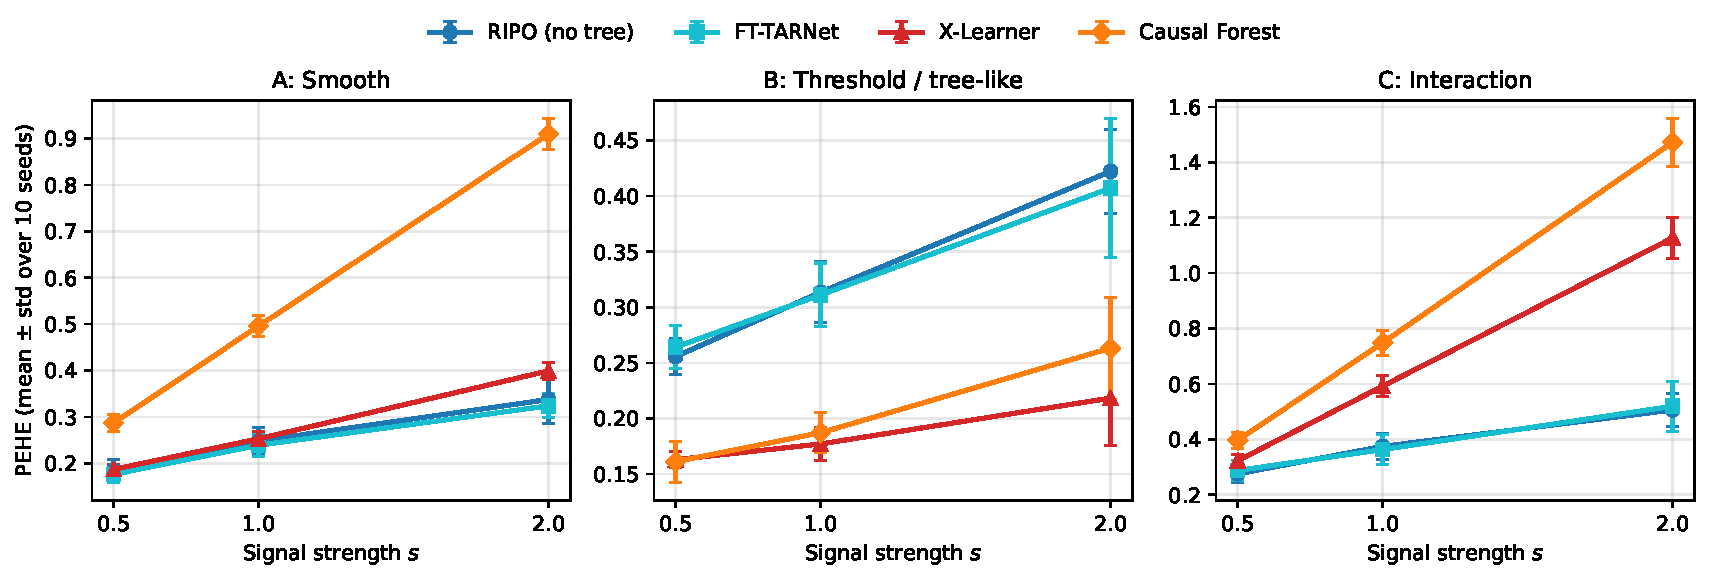
\includegraphics[width=\linewidth]{figures/paper/fig_pehe_by_regime_signal.pdf}
\caption{PEHE (mean $\pm$ std over 10~seeds) of four estimators across $\tau$-geometries and signal strengths (SPEC~v1, $n=3000$, $p=12$).}
\label{fig:regime}
\end{figure}

\begin{figure}[htbp]
\centering
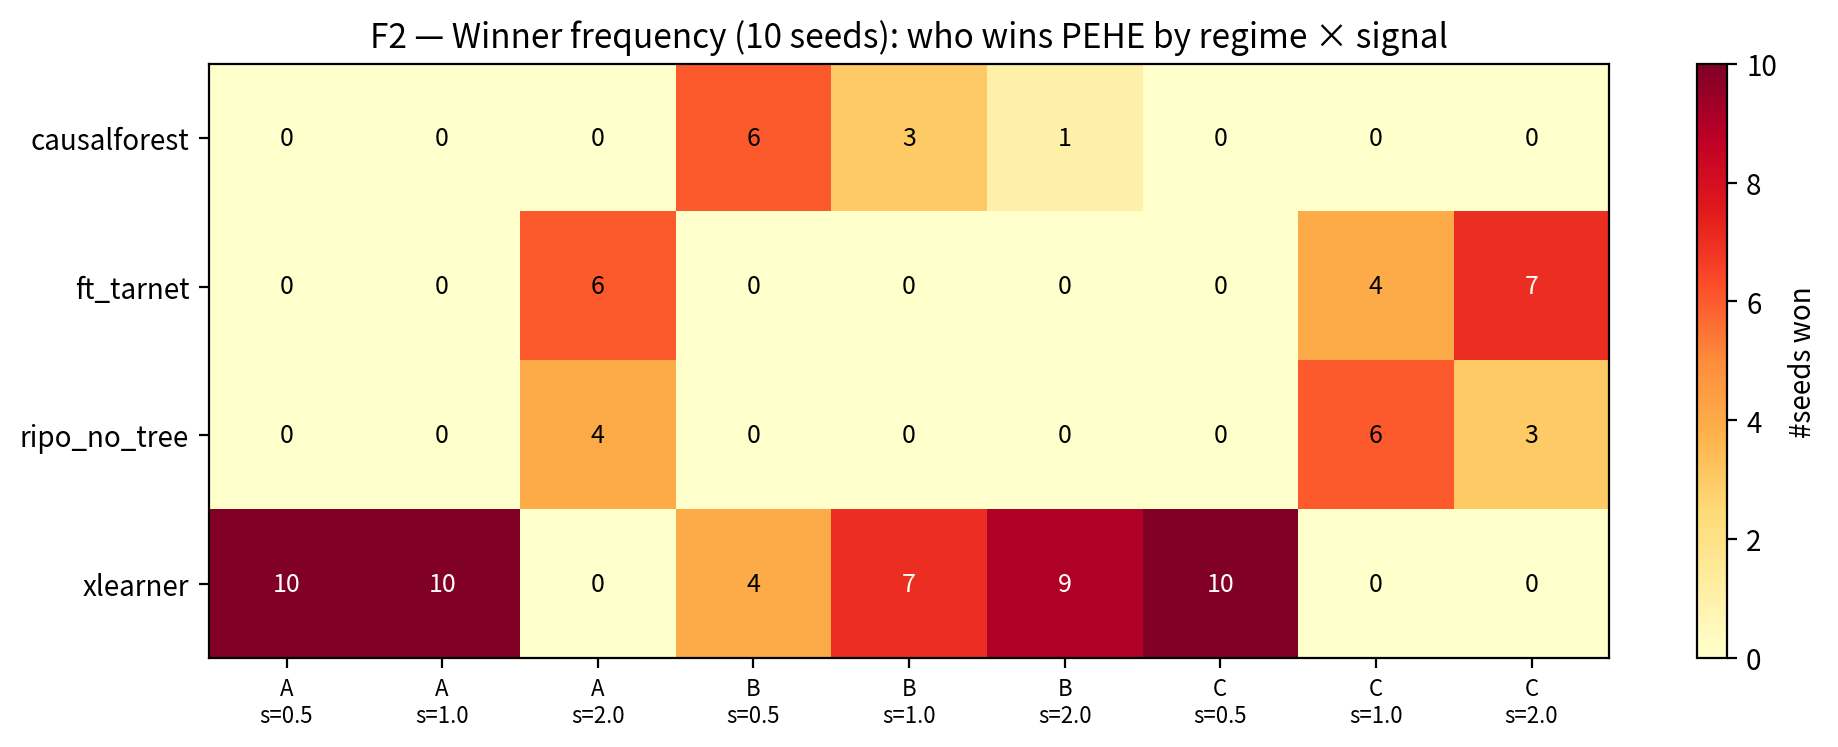
\includegraphics[width=0.9\linewidth]{figures/paper/fig_winner_freq.png}
\caption{Number of seeds (out of 10) in which each estimator has the lowest PEHE, by regime and signal $s$.}
\label{fig:winner}
\end{figure}

\begin{table}[htbp]
\centering
\caption{In-distribution PEHE ($n=3000$, $p=12$, signal~$1.0$; mean $\pm$ std over 5~seeds; lower is better). Mixture $=$ GeometryAdaptiveCATE; Avg $=$ uniform average of the two experts.}
\label{tab:indist}
\begin{tabular}{@{}lccccc@{}}
\toprule
Regime & Mixture & Neural & Tree & Avg & X-learner\\
\midrule
A (smooth)      & $0.213\pm0.011$ & $0.220\pm0.015$ & $0.237\pm0.007$ & $0.215\pm0.010$ & $0.331\pm0.016$\\
B (threshold)   & $0.281\pm0.029$ & $0.425\pm0.036$ & $0.265\pm0.027$ & $0.308\pm0.026$ & $0.265\pm0.017$\\
C (interaction) & $0.326\pm0.025$ & $0.407\pm0.065$ & $0.464\pm0.036$ & $0.336\pm0.026$ & $0.540\pm0.035$\\
\botrule
\end{tabular}
\end{table}

\begin{table}[htbp]
\centering
\caption{Ranking crossover on the smooth$\to$threshold path (10~seeds). Margin $=\PEHE_{\mathrm{tree}}-\PEHE_{\mathrm{neural}}$; positive means the neural expert is better.}
\label{tab:continuum}
\begin{tabular}{@{}cccc@{}}
\toprule
$\lambda$ & Margin (mean $\pm$ std) & Seeds neural better & Seeds tree better\\
\midrule
0.0 & $+0.016\pm0.023$ & 9/10 & 1/10\\
0.5 & $-0.056\pm0.032$ & 0/10 & 10/10\\
1.0 & $-0.141\pm0.042$ & 0/10 & 10/10\\
\botrule
\end{tabular}
\end{table}
\FloatBarrier

\subsection{Performance collapse under pure geometry shift}
\label{sec:gap}
Models trained on $\{A,B\}$ and evaluated on $C$ without adaptation reach $\PEHE=1.259\pm0.036$ (5~seeds, $n=2000$), compared with $0.326\pm0.025$ for the mixture trained and tested on $C$. The in-distribution figure is a reference only, because it comes from a model trained on $C$ with $\tau$-supervised routing.

The raw gap should be read against a constant baseline. Table~\ref{tab:gap} shows that the frozen mixture and both frozen experts are \emph{worse} than predicting the target ATE, and that routing cannot repair this: both experts fail on $C$ by almost the same amount (neural $1.283$, tree $1.249$ on average), so there is no good expert to route to. The gap is a failure of the experts to extrapolate to a new geometry, not a failure of the router.

\medskip\noindent\textbf{Consequence for the framing.} Under unconfoundedness, $\tau$ on the target is identified from target factual data $(X,T,Y)$, and a plain T-learner trained on a target factual pool of $1400$ units, with no source model, already reaches $0.47$ (Table~\ref{tab:gap}). In a setting where target factual data are available in bulk, the question is thus not one of identification but of how much target data a given strategy needs. The few-shot analysis below should be read in the regime where only $m$ target units carry usable supervision.

% --- Floats for Section 5.2 are placed here to prevent text breaks ---
\begin{table}[htbp]
\centering
\caption{Target regime $C$, shift $\{A,B\}\to C$, no adaptation (5~seeds). Reference predictors on the same test split of the target.}
\label{tab:gap}
\begin{tabular}{@{}lc@{}}
\toprule
Predictor & PEHE\\
\midrule
Frozen mixture (source-trained) & $1.259\pm0.036$\\
Frozen neural / tree expert & $1.283$ / $1.249$\\
Zero effect & $1.103\pm0.024$\\
Constant (target ATE, oracle) & $1.006\pm0.023$\\
T-learner (GBM), target factual pool only ($n=1400$; no $\tau$ labels) & $0.471\pm0.032$\\
DR-learner (GBM), target factual pool only & $0.794\pm0.066$\\
\botrule
\end{tabular}
\end{table}


\subsection{Recovery versus label budget and supervision type}
\label{sec:ladder}
We fine-tune the source model on $m\in\{10,20,30,50,100\}$ randomly selected target units under three supervision types and report PEHE on held-out target units (Table~\ref{tab:ladder}, Figure~\ref{fig:ladder}).
\begin{itemize}
  \item \textbf{Factual}: the $m$ triples $(X_i,T_i,Y_i)$ with the factual regression loss.
  \item \textbf{DR pseudo-labels}: the pseudo-outcome
  \begin{equation}
  \phi_i^{\mathrm{DR}}=\hat\mu_1(X_i)-\hat\mu_0(X_i)+\frac{T_i(Y_i-\hat\mu_1(X_i))}{\tilde e(X_i)}-\frac{(1-T_i)(Y_i-\hat\mu_0(X_i))}{1-\tilde e(X_i)}\,,
  \end{equation}
  with $\tilde e=\mathrm{clip}(e,0.05,0.95)$. In our implementation, cross-fitted ridge/logistic nuisances are fitted on the \emph{entire} target pool (including units later used for evaluation) and the pseudo-outcomes are then ridge-smoothed on $X$; only $m$ of them are used as targets. This arm is therefore \emph{transductive} and uses far more target information than $m$ units.
  \item \textbf{Oracle $\tau$}: the true $\tau$ at the $m$ units; an upper bound that is not available in practice.
\end{itemize}

We draw only the following conclusions:
\begin{enumerate}
  \item \textbf{Only oracle supervision at $m\ge 50$ clearly beats the constant baseline.} Oracle $\tau$ reaches $0.814$ at $m=50$ and $0.658$ at $m=100$, against $1.006$ for the constant. Relative to the frozen-to-in-distribution gap ($1.259\to0.326$), these correspond to roughly $48\%$ and $64\%$ of the gap; at $m=20$ it is about $18\%$.
  \item \textbf{DR stays near the constant baseline.} Its error ($0.95$--$1.00$) is flat in $m$ and has very small variance, which is consistent with a nearly global, ridge-smoothed fit rather than genuine recovery of heterogeneity. \newpage Because it is transductive, the apparent advantage of DR over oracle at $m\le 30$ is not evidence that pseudo-labels are better than true labels at a matched budget.
  \item \textbf{Small-$m$ behavior is unstable.} At $m=10$, the oracle arm is above the frozen model on average ($-0.158\pm0.300$ difference, not distinguishable from zero with $5$~seeds). In a separate run of the same shift with $n=1500$ and a different split (App.~D), the oracle arm at $m=10$ \emph{improves} ($1.116\pm0.128$ against $1.260$). We therefore do not claim that very small budgets systematically harm.
  \item \textbf{Factual fine-tuning is unreliable.} It is worse than frozen at $m=10$ and very noisy, but its mean improves on the frozen model from $m=20$ on this synthetic shift ($1.196$ at $m=20$, $0.974$ at $m=100$). On IHDP-X, it is worse than frozen for $m\le 50$ (Table~\ref{tab:ihdp}).
\end{enumerate}

\medskip\noindent\textbf{IHDP-X.} Table~\ref{tab:ihdp} and the right panel of Figure~\ref{fig:ladder} report adaptation without any gate on the semi-synthetic shift (5~replications). Frozen PEHE is $1.959\pm0.189$. When the tree signals of the frozen model are instead refitted on target outcomes, the frozen error falls to $1.552\pm0.208$ for the same shift, because the model then contains a target-only learner (Section~\ref{sec:discussion}); we do not use that protocol. The ordering of supervisions differs from the synthetic case: at $m\le 20$, the oracle arm is better than DR, whereas at $m=10$, DR does not improve on the frozen model. Oracle supervision at $m=100$ reaches $0.337$.

% --- Floats for Section 5.3 are placed here to prevent text breaks ---
\begin{table}[htbp]
\centering
\caption{Frozen model $1.259\pm0.036$, constant-ATE reference $1.006$; random selection of $m$ target units; 5~seeds. DR is transductive and not budget-matched (see text).}
\label{tab:ladder}
\begin{tabular}{@{}cccc@{}}
\toprule
$m$ & Factual & DR pseudo (transductive) & Oracle $\tau$\\
\midrule
10  & $1.436\pm0.342$ & $0.992\pm0.032$ & $1.417\pm0.297$\\
20  & $1.196\pm0.308$ & $1.001\pm0.015$ & $1.090\pm0.134$\\
30  & $1.164\pm0.085$ & $0.982\pm0.029$ & $1.098\pm0.050$\\
50  & $1.055\pm0.079$ & $0.975\pm0.020$ & $0.814\pm0.097$\\
100 & $0.974\pm0.134$ & $0.954\pm0.027$ & $0.658\pm0.069$\\
\botrule
\end{tabular}
\end{table}

\begin{figure}[!htbp]
\centering
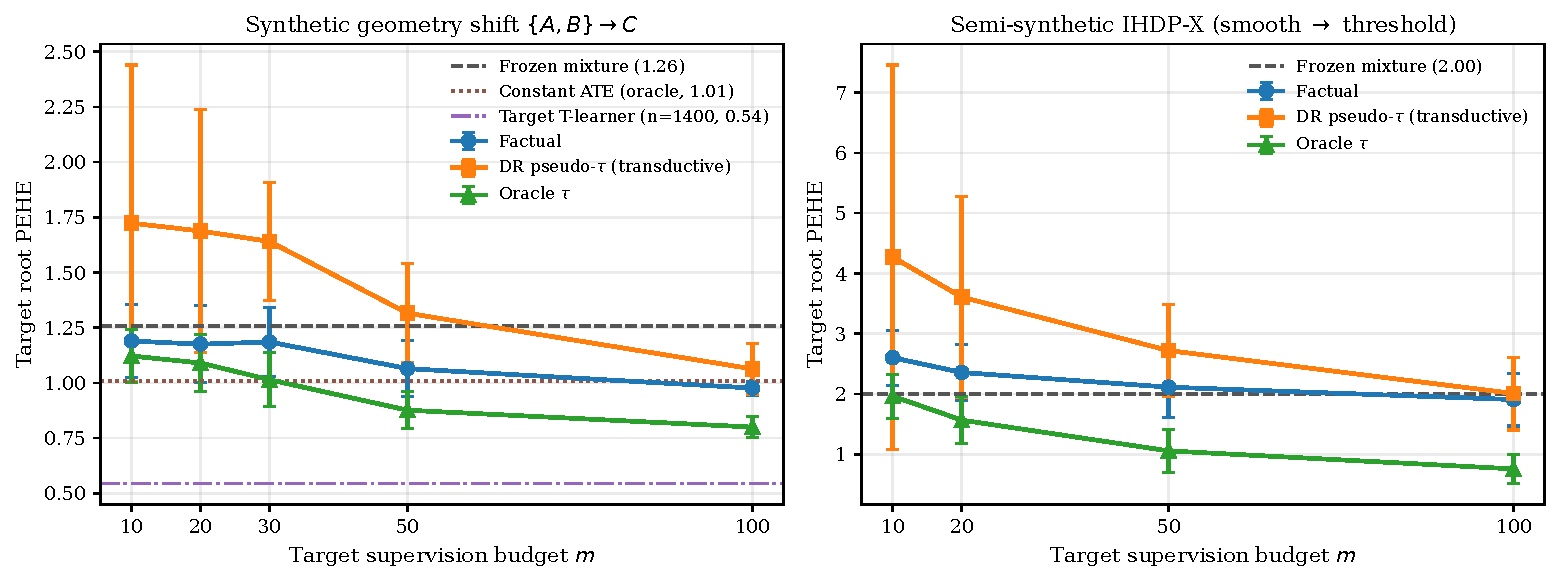
\includegraphics[width=\linewidth]{figures/paper/fig_information_ladders.pdf}
\caption{Target recovery versus label budget $m$ (random selection; mean and error bars over 5~seeds/replications). Left: synthetic $\{A,B\}\to C$ (values in Table~\ref{tab:ladder}), with the constant-ATE and target-only T-learner references of Table~\ref{tab:gap}. Right: IHDP-X, always-adapt, values of Table~\ref{tab:ihdp} (frozen $1.96$). DR pseudo-labels are transductive (see text).}
\label{fig:ladder}
\end{figure}

\FloatBarrier


\begin{table}[htbp]
\centering
\caption{IHDP-X shift (smooth$\to$threshold), always-adapt (no gate), 5~replications. $\Delta=\PEHE_{\mathrm{frozen}}-\PEHE_{\mathrm{adapted}}$; positive means improvement. Frozen $=1.959\pm0.189$.}
\label{tab:ihdp}
\begin{tabular}{@{}llcc@{}}
\toprule
$m$ & Supervision & PEHE (always-adapt) & $\Delta$\\
\midrule
10  & DR      & $2.035\pm0.214$ & $-0.076$\\
10  & Factual & $2.461\pm0.276$ & $-0.502$\\
10  & Oracle  & $1.776\pm0.278$ & $+0.183$\\
20  & DR      & $1.761\pm0.347$ & $+0.198$\\
20  & Factual & $2.687\pm0.355$ & $-0.728$\\
20  & Oracle  & $1.614\pm0.503$ & $+0.345$\\
50  & DR      & $1.546\pm0.179$ & $+0.412$\\
50  & Factual & $2.317\pm0.399$ & $-0.358$\\
50  & Oracle  & $1.172\pm0.608$ & $+0.787$\\
100 & DR      & $1.631\pm0.160$ & $+0.328$\\
100 & Factual & $1.889\pm0.337$ & $+0.070$\\
100 & Oracle  & $0.337\pm0.171$ & $+1.622$\\
\botrule
\end{tabular}
\end{table}


\subsection{Negative results}
\label{sec:neg}
\medskip\noindent\textbf{Source-trained observable routers.} In a separate router-transfer study (10~seeds; Table~\ref{tab:router}), four base estimators (residual-attention, FT-TARNet, X-learner, causal forest) are fitted on each regime's own data, and a router over observable prediction-based features is trained on a source regime and applied to a target regime. On every source--target pair and signal level in the study, the router is worse on the target than the best single base estimator, selected in hindsight, and the deficit grows with signal and for the hardest pair ($B\to C$, signal $2.0$: $1.029$ vs.\ $0.437$); it is also far from the pointwise oracle choice (Figures~\ref{fig:e3} and~\ref{fig:e1}). This study is separate from the $\{A,B\}\to C$ shift above, where routing has no headroom because both experts fail.

\medskip\noindent\textbf{Observable geometry score.} A train-only geometry score tracks the performance margin between tree-based and neural estimators on the synthetic continuum (Pearson $r=-0.71$, 25~rows from 5~seeds), but on ACIC settings 1, 2, 3, 4, 5, 8 (3~seeds), its winner-prediction accuracy is $0.61$, below the majority-class baseline of $0.78$. ACIC settings 2 and 3 have essentially zero correlation between estimated and true CATE for all methods (no resolvable heterogeneity), so they should not be used as evidence about $\tau$-geometry; we exclude them from any geometry argument.

\medskip\noindent\textbf{Active acquisition.} Selecting target units by disagreement/entropy (active hybrid) does not beat random selection in our ladder: e.g., oracle at $m=50$ gives $1.193\pm0.308$ (active) against $0.814\pm0.097$ (random), and DR at $m=10$ gives $1.165\pm0.167$ against $0.992\pm0.032$.

\medskip\noindent\textbf{Real benchmarks.} On canonical IHDP, a related residual-attention model (RIPO, not the mixture above) reaches $0.157\pm0.047$ with outcomes rescaled by the loader, comparable to a feature-tokenizer TARNet ($0.182\pm0.074$) and clearly better than the X-learner ($0.464\pm0.163$); because of the rescaling, these values are not comparable to published IHDP numbers. On ACIC settings 1, 4, 5, 8, the mixture is competitive but not dominant (App.~C).

% --- Floats for Section 5.4 are placed here to prevent text breaks ---
\begin{table}[htbp]
\centering
\caption{Router-transfer study, signal~$1.0$, 10~seeds, PEHE on the target regime. Router: observable router trained on the source regime. Global: best single base estimator on the target, chosen in hindsight. Oracle: pointwise best of the four base estimators (uses true $\tau$).}
\label{tab:router}
\begin{tabular}{@{}cccc@{}}
\toprule
Source$\to$Target & Router & Global & Oracle\\
\midrule
A$\to$B & 0.263 & 0.170 & 0.094\\
A$\to$C & 0.483 & 0.391 & 0.206\\
B$\to$A & 0.404 & 0.252 & 0.137\\
B$\to$C & 0.619 & 0.391 & 0.206\\
\botrule
\end{tabular}
\end{table}

\begin{figure}[htbp]
\centering
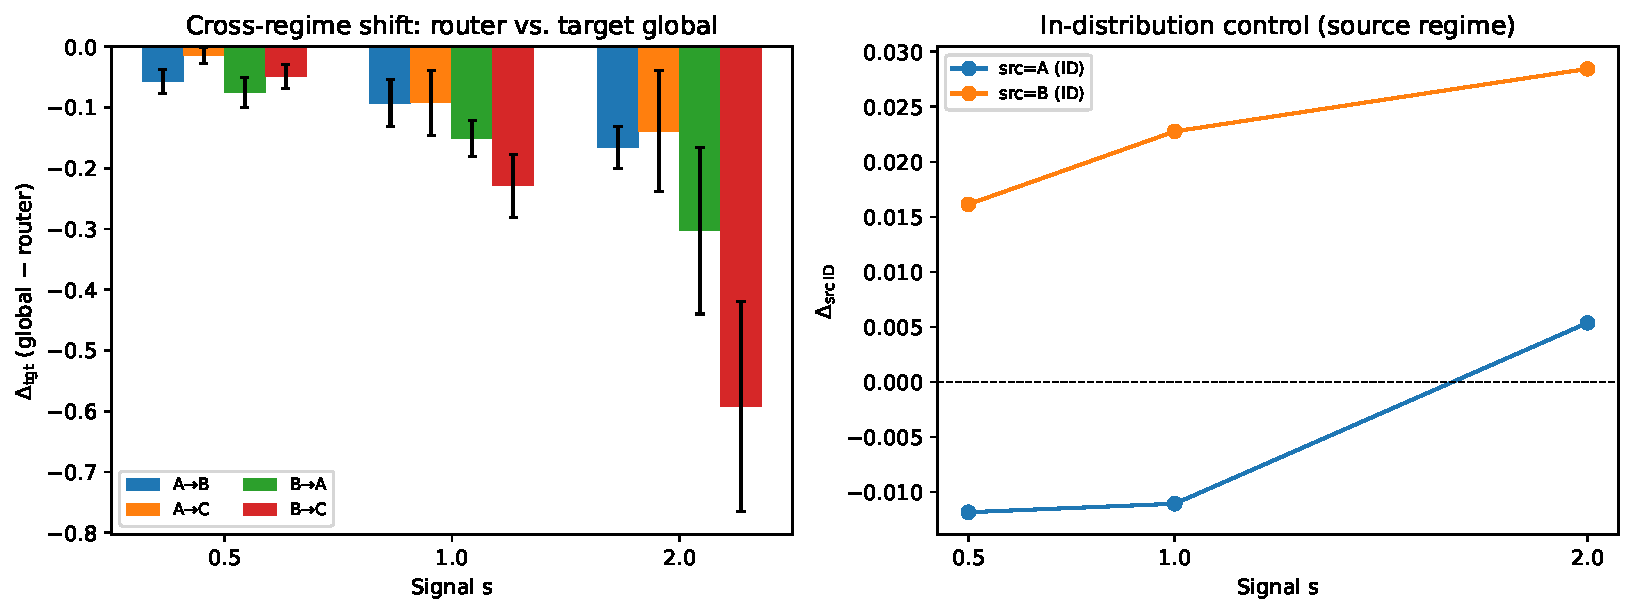
\includegraphics[width=\linewidth]{figures/paper/fig_e3_shift.pdf}
\caption{Left: $\Delta_{\mathrm{tgt}}=\PEHE_{\mathrm{global}}-\PEHE_{\mathrm{router}}$ on the target regime (negative: the source-trained router is worse than the best single estimator). Right: in-distribution control (source regime), where the router is close to the global estimator.}
\label{fig:e3}
\end{figure}

\begin{figure}[!htbp]
\centering
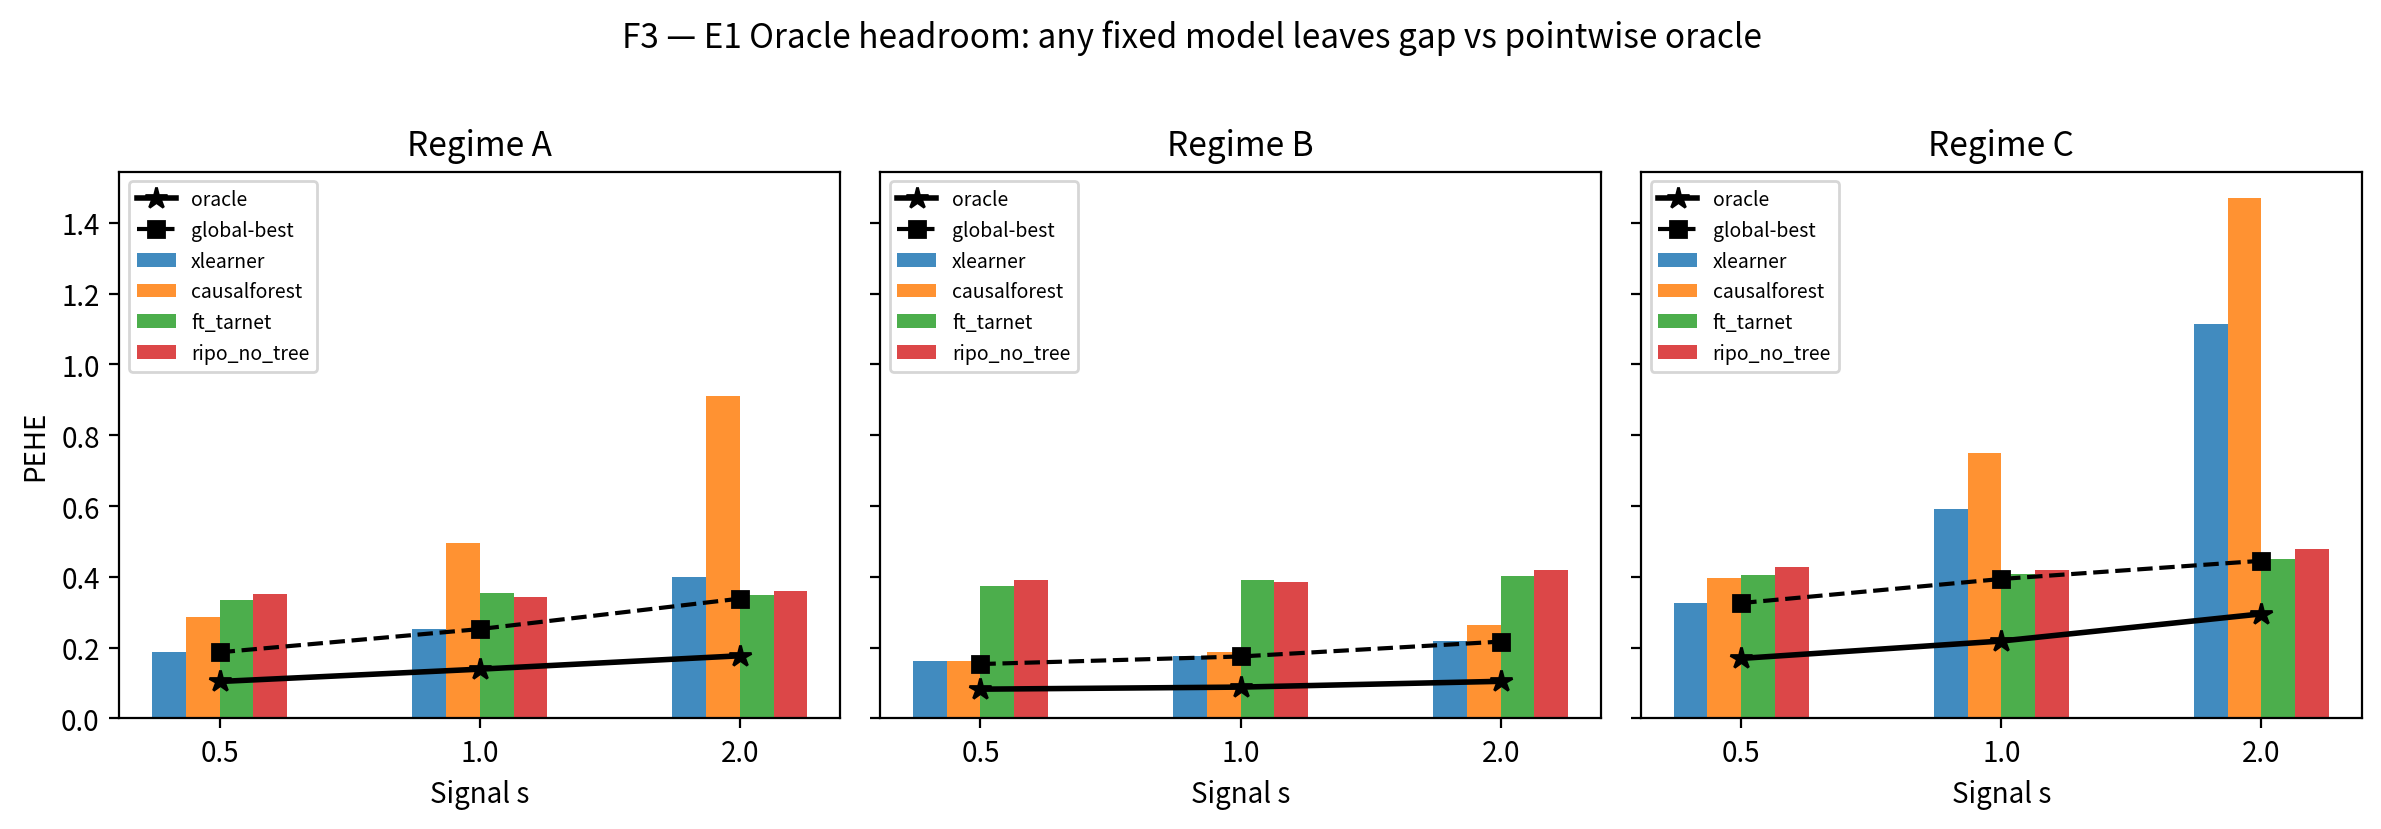
\includegraphics[width=\linewidth]{figures/paper/fig_e1_oracle_gap.png}
\caption{Oracle headroom: the pointwise best of four estimators (``oracle'', uses true $\tau$) is much better than any fixed estimator (``global-best''), in every regime and signal. This headroom is what a router would have to capture from observable information alone.}
\label{fig:e1}
\end{figure}

\FloatBarrier

%--------------------------------------------------------------------
\section{Discussion and limitations}
\label{sec:discussion}
\begin{itemize}
  \item \textbf{Scope.} The shift and adaptation evidence is synthetic or semi-synthetic, uses 5~seeds/replications, and compares one two-expert architecture. With 5~seeds, the smallest attainable two-sided Wilcoxon $p$-value is $0.0625$, so we report means, spreads, and win counts rather than significance. The ranking-reversal evidence (10~seeds) is stronger.
  \item \textbf{Oracle supervision.} Counterfactual labels are unavailable in practice. The oracle arm is an information bound, not a protocol.
  \item \textbf{Unequal budgets.} DR pseudo-labels are built from the whole target pool, whereas factual and oracle arms use only $m$ units. A budget-matched comparison and learners trained from scratch on the same pool are needed before conclusions about pseudo-label quality can be drawn; the T-learner baseline in Table~\ref{tab:gap} indicates that these comparisons can change the picture.
  \item \textbf{Instrument.} Stage-2 routing on synthetic sources uses $\tau$ supervision; the mixture is a measurement device rather than a competing estimator.
  \item \textbf{Target leakage in the frozen baseline.} If the tree signals fed to the frozen model are cross-fitted on target outcomes, the model is no longer source-only: the frozen error drops from $1.259$ to $0.523$ on $\{A,B\}\to C$ and from $1.959$ to $1.552$ on IHDP-X, and any comparison with learners trained from a few target points becomes unfair. All reported numbers use tree models fitted on source data only.
  \item \textbf{IHDP-X} shares covariates between source and target and uses re-simulated outcomes.
  \item \textbf{Theory.} We provide no formal guarantees; any structural arguments are informal.
\end{itemize}

\section{Conclusion}
CATE estimator rankings reverse with the geometry of $\tau$, standard $\tau$-free surrogates are less reliable on interaction surfaces, and, on our synthetic shift, a model trained on other geometries is worse than a constant predictor on a new one. Recovery from a few target units depends strongly on supervision type and on how the comparison is set up; only oracle supervision at moderate budgets clearly helps in our experiments, and simple learners fit on the target factual pool can do better than any few-shot adaptation we tested. Observable routers and geometry scores do not close the gap. These results are a characterization and a cautionary protocol study; a budget-matched, deployable treatment of adaptation is left to future work.

\backmatter

\section*{Declarations}
\begin{itemize}
\item \textbf{Funding:} The authors declare that no funds, grants, or other support were received during the preparation of this manuscript.
\item \textbf{Conflict of interest:} The authors have no relevant financial or non-financial interests to disclose.
\item \textbf{Ethics approval:} Not applicable.
\item \textbf{Consent to participate:} Not applicable.
\item \textbf{Consent for publication:} Not applicable.
\item \textbf{Availability of data and materials:} The datasets generated during and/or analysed during the current study are available in the accompanying GitHub repository: \url{https://github.com/YOUR-USERNAME/cate-geometry-shift}.
\item \textbf{Code availability:} The source code is available in the accompanying GitHub repository: \url{https://github.com/YOUR-USERNAME/cate-geometry-shift}.
\item \textbf{Authors' contributions:} Both authors contributed equally to this work.
\end{itemize}

\begin{appendices}
\section{Hard design and PEHE decomposition}
\label{app:hard}
Hard design ($n=5000$, $p=50$, $\sigma=1$, 10~seeds): $\Delta=\PEHE_{\mathrm{neural}}-\PEHE_{\mathrm{X}}$; negative means the X-learner is better.

\begin{table}[htbp]
\centering
\caption{Hard design PEHE across regimes and signals.}
\label{tab:hard_design}
\begin{tabular}{@{}lcccc@{}}
\toprule
Regime & Signal & Neural & X-learner & $\Delta$\\
\midrule
A & 0.5 & 0.269 & 0.263 & $-$0.006\\
A & 1.0 & 0.368 & 0.319 & $-$0.048\\
A & 2.0 & 0.512 & 0.436 & $-$0.076\\
B & 0.5 & 0.317 & 0.246 & $-$0.071\\
B & 1.0 & 0.423 & 0.257 & $-$0.166\\
B & 2.0 & 0.541 & 0.274 & $-$0.268\\
C & 0.5 & 0.422 & 0.390 & $-$0.032\\
C & 1.0 & 0.522 & 0.640 & $+$0.118\\
C & 2.0 & 0.695 & 1.159 & $+$0.463\\
\botrule
\end{tabular}
\end{table}

Turning the mean-difference balancing penalty on lowers PEHE mainly at signal~$0.5$ ($-0.079$, $-0.054$, $-0.062$ on $A$, $B$, and $C$), and by a small margin at higher signals; the change is driven by lower outcome-model errors rather than by the PEHE cross-term.

\section{Surrogate-selection accuracy by geometry}
\label{app:surr}
Four CATE estimators are scored with $\tau$-free surrogates; ``oracle'' is the lowest-PEHE estimator (30~cells per regime: 10~seeds $\times$ 3~signals).

\begin{table}[htbp]
\centering
\caption{Surrogate-selection accuracy and mean regret across geometries.}
\label{tab:surrogate_selection}
\begin{tabular}{@{}lcccccc@{}}
\toprule
 & \multicolumn{3}{c}{Selection accuracy} & \multicolumn{3}{c}{Mean regret}\\
Surrogate & A & B & C & A & B & C\\
\midrule
Random & 0.23 & 0.23 & 0.17 & 0.145 & 0.123 & 0.212\\
Factual MSE & 0.90 & 0.93 & 0.70 & 0.002 & 0.001 & 0.009\\
IPW residual & 0.90 & 0.93 & 0.60 & 0.002 & 0.001 & 0.017\\
Pseudo-DR & 0.83 & 0.87 & 0.63 & 0.010 & 0.003 & 0.015\\
Policy proxy & 0.53 & 0.53 & 0.43 & 0.039 & 0.058 & 0.031\\
$-\mathrm{Var}(\hat\tau)$ & 0.10 & 0.00 & 0.33 & 0.082 & 0.226 & 0.056\\
\botrule
\end{tabular}
\end{table}

\section{ACIC benchmark}
\label{app:acic}
PEHE (mean over 5~replications) on settings with measurable heterogeneity: setting~1: mixture $0.943$, X-learner $0.869$; setting~4: $1.222$, $1.444$; setting~5: $1.078$, $1.441$; setting~8: all methods near $2.8$ with large spread. The mixture is competitive but not dominant. Settings 2 and 3 (near-constant effects) are excluded from geometry conclusions.

\section{An oracle-calibrated adaptation gate (exploratory, not recommended for deployment)}
\label{app:gate}
We also evaluated a rule that adapts only if an estimated target error plus a penalty $c/\sqrt m$ is below the estimated frozen error minus a margin $\gamma$. In our code, the estimated errors are computed against the \emph{true} $\tau$ on a calibration slice, so the gate is an oracle-calibrated benchmark rather than a deployable procedure. On IHDP-X, the decision for factual supervision is a hard rule (freeze unless $m\ge 80$ and a holdout improvement exists) and for oracle supervision a hard rule (freeze if $m<25$); these rules were adjusted after an earlier smoke run. Consequently, the observation that the gate ``blocks'' factual updates is built into the rule and is not an empirical finding, and we do not present the gate as a contribution. In the synthetic $\{A,B\}\to C$ run with this gate ($n=1500$), the deployable proxy variant never adapted under oracle supervision.

\section*{Reproducibility}
Seeds, configurations, and code are in the project repository. \path{supp_baselines.py} reproduces the zero, constant, and target-only learner baselines of Table~\ref{tab:gap} (zero $1.103$, constant $1.006$, T-learner $0.471$, DR-learner $0.794$). The random selection of target units in the repository uses Python's \texttt{hash} on a string, so exact subsets can differ between runs unless \texttt{PYTHONHASHSEED} is fixed; the reported means are over five seeds.
\end{appendices}

\begin{thebibliography}{99}
\bibitem[Alaa and van der Schaar(2019)]{alaa2019} Alaa, A., van der Schaar, M., 2019. Validating causal inference models via influence functions. In: Proc.\ ICML, PMLR 97, pp.\ 191--201.
\bibitem[Athey et al.(2019)]{athey2019} Athey, S., Tibshirani, J., Wager, S., 2019. Generalized random forests. Ann.\ Statist.\ 47(2), 1148--1178.
\bibitem[Bareinboim and Pearl(2016)]{bareinboim2016} Bareinboim, E., Pearl, J., 2016. Causal inference and the data-fusion problem. Proc.\ Natl.\ Acad.\ Sci.\ 113(27), 7345--7352.
\bibitem[Dahabreh et al.(2019)]{dahabreh2019} Dahabreh, I.J., Robertson, S.E., Tchetgen Tchetgen, E.J., Stuart, E.A., Hern\'an, M.A., 2019. Generalizing causal inferences from individuals in randomized trials to all trial-eligible individuals. Biometrics 75(2), 685--694.
\bibitem[Grinsztajn et al.(2022)]{grinsztajn2022} Grinsztajn, L., Oyallon, E., Varoquaux, G., 2022. Why do tree-based models still outperform deep learning on typical tabular data? In: Advances in Neural Information Processing Systems 35 (Datasets and Benchmarks Track).
\bibitem[K\"unzel et al.(2018)]{kunzel2018} K\"unzel, S.R., Stadie, B.C., Vemuri, N., Ramakrishnan, V., Sekhon, J.S., Abbeel, P., 2018. Transfer learning for estimating causal effects using neural networks. arXiv:1808.07804.
\bibitem[Rolling and Yang(2014)]{rolling2014} Rolling, C.A., Yang, Y., 2014. Model selection for estimating treatment effects. J.\ R.\ Stat.\ Soc.\ Ser.\ B 76(4), 749--769.
\bibitem[Saito and Yasui(2020)]{saito2020} Saito, Y., Yasui, S., 2020. Counterfactual cross-validation: stable model selection procedure for causal inference models. In: Proc.\ ICML, PMLR 119, pp.\ 8398--8407.
\bibitem[Chipman et al.(2010)]{chipman2010} Chipman, H.A., George, E.I., McCulloch, R.E., 2010. BART: Bayesian additive regression trees. Ann.\ Appl.\ Statist.\ 4(1), 266--298.
\bibitem[Curth and van der Schaar(2021)]{curth2021} Curth, A., van der Schaar, M., 2021. On inductive biases for heterogeneous treatment effect estimation. In: Advances in Neural Information Processing Systems 34.
\bibitem[Curth et al.(2021)]{curth2021benchmark} Curth, A., Svensson, D., Weatherall, J., van der Schaar, M., 2021. Really doing great at estimating CATE? A critical look at ML benchmarking practices in treatment effect estimation. In: Proc.\ NeurIPS Datasets and Benchmarks Track.
\bibitem[Dorie et al.(2019)]{dorie2019} Dorie, V., Hill, J., Shalit, U., Scott, M., Cervone, D., 2019. Automated versus do-it-yourself methods for causal inference: lessons learned from a data analysis competition. Statist.\ Sci.\ 34(1), 43--68.
\bibitem[Hill(2011)]{hill2011} Hill, J.L., 2011. Bayesian nonparametric modeling for causal inference. J.\ Comput.\ Graph.\ Statist.\ 20(1), 217--240.
\bibitem[Johansson et al.(2016)]{johansson2016} Johansson, F.D., Shalit, U., Sontag, D., 2016. Learning representations for counterfactual inference. In: Proc.\ ICML, pp.\ 3020--3029.
\bibitem[Kennedy(2023)]{kennedy2023} Kennedy, E.H., 2023. Towards optimal doubly robust estimation of heterogeneous causal effects. Electron.\ J.\ Statist.\ 17(2), 3008--3049.
\bibitem[K\"unzel et al.(2019)]{kunzel2019} K\"unzel, S.R., Sekhon, J.S., Bickel, P.J., Yu, B., 2019. Metalearners for estimating heterogeneous treatment effects using machine learning. Proc.\ Natl.\ Acad.\ Sci.\ 116(10), 4156--4165.
\bibitem[Kyono et al.(2023)]{kyono2023} Kyono, T., Bica, I., Qian, Z., van der Schaar, M., 2023. Selecting treatment effects models for domain adaptation using causal knowledge. ACM Trans.\ Comput.\ Healthcare 4(2), 1--29.
\bibitem[Mahajan et al.(2024)]{mahajan2024} Mahajan, D., Mitliagkas, I., Neal, B., Syrgkanis, V., 2024. Empirical analysis of model selection for heterogeneous causal effect estimation. In: Proc.\ ICLR.
\bibitem[Nie and Wager(2021)]{nie2021} Nie, X., Wager, S., 2021. Quasi-oracle estimation of heterogeneous treatment effects. Biometrika 108(2), 299--319.
\bibitem[Pearl and Bareinboim(2011)]{pearl2011} Pearl, J., Bareinboim, E., 2011. Transportability of causal and statistical relations: a formal approach. In: Proc.\ AAAI, pp.\ 247--254.
\bibitem[Schuler et al.(2018)]{schuler2018} Schuler, A., Baiocchi, M., Tibshirani, R., Shah, N., 2018. A comparison of methods for model selection when estimating individual treatment effects. arXiv:1804.05146.
\bibitem[Shalit et al.(2017)]{shalit2017} Shalit, U., Johansson, F.D., Sontag, D., 2017. Estimating individual treatment effect: generalization bounds and algorithms. In: Proc.\ ICML, PMLR 70, pp.\ 3076--3085.
\bibitem[Shi et al.(2019)]{shi2019} Shi, C., Blei, D., Veitch, V., 2019. Adapting neural networks for the estimation of treatment effects. In: Advances in Neural Information Processing Systems 32, pp.\ 2503--2513.
\bibitem[Wager and Athey(2018)]{wager2018} Wager, S., Athey, S., 2018. Estimation and inference of heterogeneous treatment effects using random forests. J.\ Amer.\ Statist.\ Assoc.\ 113(523), 1228--1242.
\end{thebibliography}

\end{document}
